\section{Identification du sens du résultat}
\subsection{Contexte}
\begin{frame}{Contexte}	
\begin{itemize}	\small
	\item Uniquement les décisions à une demande de la catégorie
	\begin{itemize}\scriptsize
		\item Raison: plus de $50\%$ des documents dans la majorité des catégories
	\end{itemize}
	\item Classification binaire (éviter les subtilités de rédaction)
	\begin{itemize} \scriptsize
		\item Raison: les demandes sont en majorité \textbf{acceptées} ou \textbf{rejetées}
	\end{itemize}
\end{itemize}
\centering 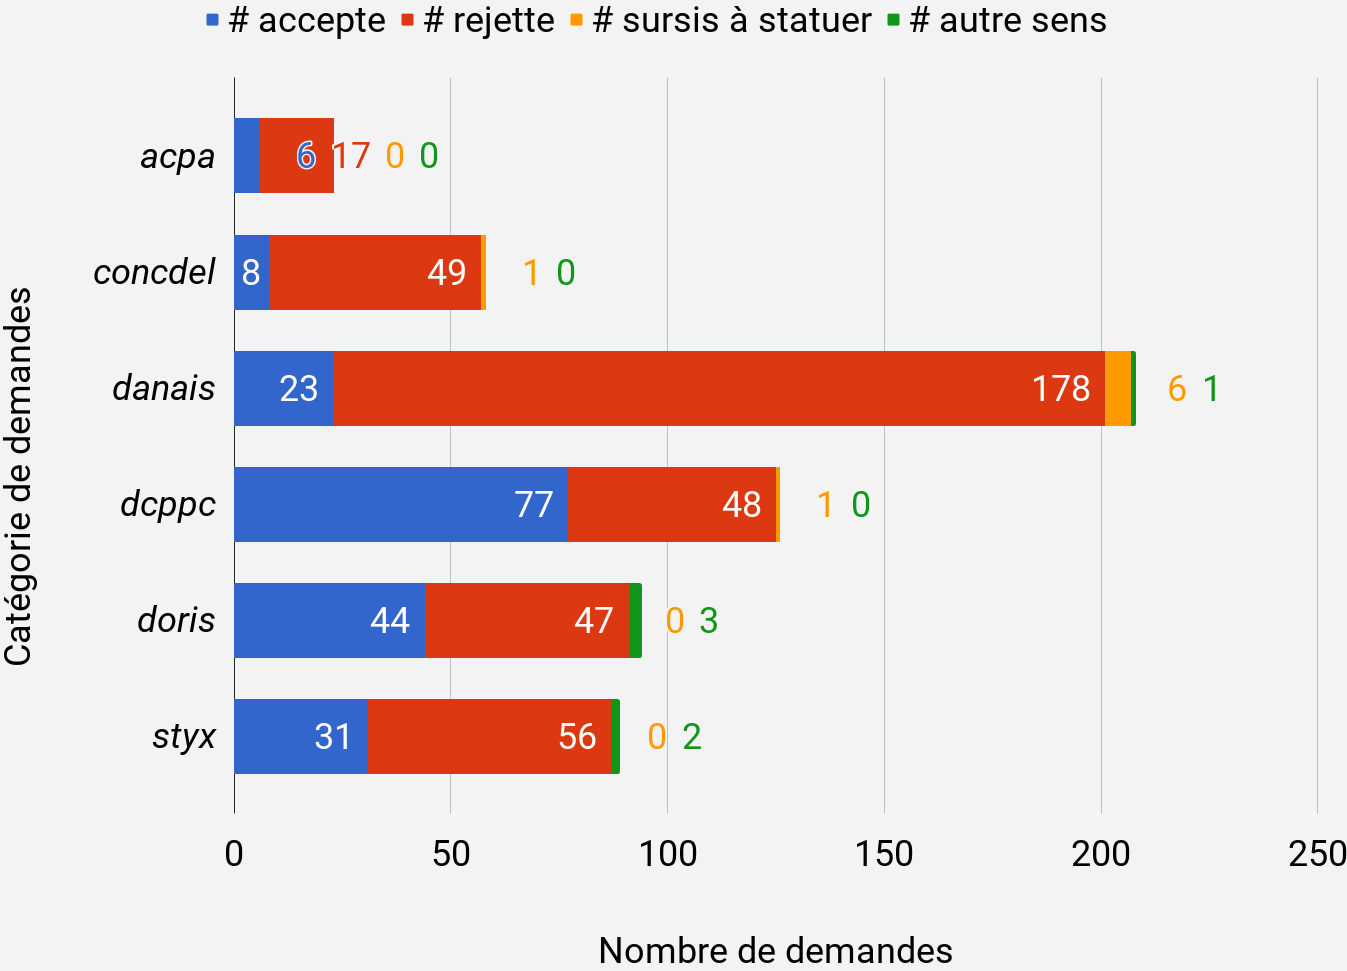
\includegraphics[width=0.7\textwidth]{chartDistrSens.png}
\end{frame}

\subsection{Bibliographie : algorithmes classiques}

\begin{frame}{Bibliographie : algorithmes classiques}
	\begin{itemize}
		\item Classifieur bayésien naïf
		\item K-plus-proches-voisins
		\item SVM
		\item Arbre de décision
		\item Analyse discriminante linéaire et quadratique
		\item NBSVM \cite{wang2012nbsvm}
		\item fastText \cite{grave2017fasttextcls}		
	\end{itemize}
\end{frame}

\begin{frame}{Résultats obtenus avec fastText et NBSVM}

\begin{table}[htb]
	\tiny
	\begin{center}
		\begin{tabular}{|c|c|c|c|c|c|c|c|c|}
			\hline
			Cat. Dmd. & Algo. & {Préc.} & {Préc. équi.} & {err-0} & {err-1} & $F_1(0)$ & $F_1(1)$ & {$F_{1macro}$} \\ \hline
			\textit{dcppc} & NBSVM & 0.875 & 0.812 & 0 & 0.375 & 0.916 & 0.752 & \textbf{0.834} \\ \hline
			\textit{danais} & fastText & 0.888 & 0.5 & 0 & 1 & 0.941 & 0 & 0.47 \\ \hline
			\textit{danais} & NBSVM & 0.888 & 0.5 & 0 & 1 & 0.941 & 0 & 0.47 \\ \hline
			\textit{concdel} & fastText & 0.775 & 0.5 & 0 & 1 & 0.853 & 0 & 0.437 \\ \hline
			\textit{concdel} & NBSVM & 0.775 & 0.5 & 0 & 1 & 0.873 & 0 & 0.437 \\ \hline
			\textit{acpa} & fastText & 0.745 & 0.5 & 0 & 1 & 0.853 & 0 & 0.426 \\ \hline
			\textit{acpa} & NBSVM & 0.745 & 0.5 & 0 & 1 & 0.853 & 0 & 0.426 \\ \hline
			\textit{doris} & NBSVM & 0.5 & 0.492 & 0.167 & 0.85 & 0.63 & 0.174 & 0.402 \\ \hline
			\textit{dcppc} & fastText & 0.667 & 0.5 & 0 & 1 & 0.8 & 0 & 0.4 \\ \hline
			\textit{styx} & fastText & 0.667 & 0.5 & 0 & 1 & 0.8 & 0 & 0.4 \\ \hline
			\textit{styx} & NBSVM & 0.667 & 0.5 & 0 & 1 & 0.8 & 0 & 0.4 \\ \hline
			\textit{doris} & fastText & 0.523 & 0.5 & 0 & 1 & 0.686 & 0 & 0.343 \\ \hline
		\end{tabular}
	\end{center}
0 = "rejette" et 1 == "accepte"
\end{table}
\scriptsize
\textbf{Influence du déséquilibre et de la (très) faible taille des données}
\end{frame}

\begin{frame}{Application des extensions de la Régression PLS (1)}
PLS standard (Régression partielle des moindres carrés) 

Réduction supervisée des dimensions $x_1, x_2, ..., x_p$ en composantes orthogonales $t_1, ...., t_h$

$t_h = w_{h1} x_1 + \cdots + w_{hj} x_j + \cdots + w_{hp} x_p$

avec $w_{hj} = \frac{cov(u_{(h-1)j}, \epsilon_h)}{\sqrt{\sum_p^{j=1} cov^2(u_{(h-1)j}, \epsilon_h)}}$
, $y=c_1 t_1 + ... + c_h t_h + \epsilon_h$,

et $x_j=\beta_{1j} t_1 + ... + \beta_{hj} t_h + u_{(h-1)j}$


\end{frame}

\begin{frame}{Application des extensions de la Régression PLS (2)}

\begin{enumerate}
\setlength\itemsep{1.5em}

\item Gini-PLS: 
élimination de la sensibilité au \textit{outliers} en remplaçant la covariance $cov(x_j, y)$ par la covariance de Gini $cog(y; x_j) := cov(y; R(x_j))$ pour l'estimation des résidus $u_{(h)j}$ et des poids $w_{hj}$ \cite{mussard2018ginipls}

\item Logit-PLS:  $\forall j > 1$, les $w_{hj} $ sont les coefficients de la régression logistique de $y$ sur les composantes $t_1, ..., t_{h-1}, u_{(h-1)j}$ \cite{tenenhaus2005logitpls}

\item Gini-Logit-PLS: covariance Gini pour $u_{(h)j}$ et coefficient Logit pour les $w_{hj}$
\end{enumerate}
\end{frame}


\begin{frame}{Résultats: classifieurs PLS vs. aux arbres de décision}
\begin{table}[]
\tiny
\label{my-label}
\begin{tabular}{|l|l|l|l|l|l|l|l|l|l|}
\hline
\textbf{Vecteur} & \textbf{classifieur} & \textbf{F1} & \textbf{min} & \textbf{Cat. min} & \textbf{max} & \textbf{Cat. max} & \textbf{F1 - 1$^{er}$F1} & \textbf{max - min} & \textbf{rang} \\ \hline
GSS*TF                 & Tree                & \textbf{0.668}     & 0.5                 & doris                  & 0.92               & dcppc                 & \textbf{0}                    & \textbf{0.42}           & 1             \\ \hline
AVG-G*TF      & LogitPLS         & \textbf{0.648}     & 0.518               & danais                 & 0.781              & dcppc                 & \textbf{0.02}                 & \textbf{0.263}          & 13            \\ \hline
AVG-G*TF      & StandardPLS      & \textbf{0.636}     & 0.49                & danais                 & 0.836              & dcppc                 & \textbf{0.032}                & \textbf{0.346}          & 24            \\ \hline
DELTADF*TF             & GiniPLS          & \textbf{0.586}     & 0.411               & danais                 & 0.837              & dcppc                 & \textbf{0.082}                & \textbf{0.426}          & 169           \\ \hline
DELTADF*TF             & GiniLogitPLS     & \textbf{0.578}     & 0.225               & styx                   & 0.772              & dcppc                 & \textbf{0.09}                 & \textbf{0.547}          & 220           \\ \hline
\end{tabular}
AVG-G == Moyenne des métriques globales de pondération
\end{table}
\scriptsize

Les extensions du PLS ne sont pas très éloignées (si on choisi le bon shéma de vectorisation)

\end{frame}

\begin{frame}{Résultats : restriction de régions du document}
\begin{table}[]
\tiny
\centering
\label{my-label}
\begin{tabular}{|l|l|l|l|l|}
\hline
\textbf{Cat. Dmd} & \textbf{zone}                                    & \textbf{Vecteur}      & \textbf{classifieur} & \textbf{F1}    \\ \hline
\textbf{acpa}     & \textbf{demande\_resultat\_a\_resultat\_context} & \textbf{DBIDF*TF}           & \textbf{Tree}        & \textbf{0.846} \\ \hline
acpa              & litige\_motifs\_dispositif                       & DELTADF*TF                  & StandardPLS       & 0.697          \\ \hline
acpa              & litige\_motifs\_dispositif                       & AVERAGEGlobals*TF           & LogitPLS          & 0.683          \\ \hline
\textbf{concdel}  & \textbf{litige\_motifs\_dispositif}              & \textbf{GSS*TF}             & \textbf{Tree}        & \textbf{0.798} \\ \hline
concdel           & motifs                                           & IDF*TF                      & GiniLogitPLS      & 0.703          \\ \hline
concdel           & context                                          & DBIDF*LOGAVE                & StandardPLS       & 0.657          \\ \hline
\textbf{danais}   & \textbf{demande\_resultat\_a\_resultat\_context} & \textbf{CHI2*AVERAGELocals} & \textbf{Tree}        & \textbf{0.813} \\ \hline
danais            & demande\_resultat\_a\_resultat\_context          & AVERAGEGlobals*ATF          & LogitPLS          & 0.721          \\ \hline
danais            & demande\_resultat\_a\_resultat\_context          & AVERAGEGlobals*ATF          & StandardPLS       & 0.695          \\ \hline
\textbf{dcppc}    & \textbf{demande\_resultat\_a\_resultat\_context} & \textbf{CHI2*TF}            & \textbf{Tree}        & \textbf{0.985} \\ \hline
dcppc             & demande\_resultat\_a\_resultat\_context          & CHI2*TF                     & LogitPLS          & 0.94           \\ \hline
dcppc             & litige\_motifs\_dispositif                       & MARASCUILO*TP               & StandardPLS       & 0.934          \\ \hline
\textbf{doris}    & \textbf{litige\_motifs\_dispositif}              & \textbf{DSIDF*TP}           & \textbf{GiniPLS}  & \textbf{0.806} \\ \hline
doris             & litige\_motifs\_dispositif                       & DSIDF*TP                    & GiniLogitPLS      & 0.806          \\ \hline
doris             & litige\_motifs\_dispositif                       & IG*ATF                      & StandardPLS       & 0.772          \\ \hline
\textbf{styx}     & \textbf{motifs}                                  & \textbf{DSIDF*TF}           & \textbf{Tree}        & \textbf{1}     \\ \hline
styx              & demande\_resultat\_a\_resultat\_context          & DSIDF*LOGAVE                & GiniLogitPLS      & 0.917          \\ \hline
styx              & litige\_motifs\_dispositif                       & RF*TF                       & GiniPLS           & 0.833          \\ \hline
\end{tabular}
\end{table}

Les résultats s'améliorent si ont exploite la zone adéquate pour la catégorie
\end{frame}